\documentclass[10pt]{beamer}

\usetheme{metropolis}
\usepackage{appendixnumberbeamer}

\usepackage{booktabs}
\usepackage[scale=2]{ccicons}
\usepackage{graphicx}
\usepackage{hyperref}
\usepackage{circuitikz}
\usepackage{pdflscape}
\usepackage{smartdiagram}

\usepackage{color}
\usepackage{listings}

\lstset{
	basicstyle=\footnotesize\ttfamily,
    keepspaces=true,
    showstringspaces=false,
    language=PHP,
    commentstyle=\ttfamily,
}

\usepackage[OT4]{polski}
\usepackage[utf8]{inputenc}

\usepackage{pgfplots}
\usepgfplotslibrary{dateplot}

\usepackage{xspace}
\newcommand{\themename}{\textbf{\textsc{metropolis}}\xspace}

\setbeamertemplate{frame footer}{}
\setbeamertemplate{frame numbering}{}

\usetikzlibrary{shapes,arrows}

\tikzstyle{decision} = [diamond, draw, fill=blue!20, 
    text width=4.5em, text badly centered, node distance=3cm, inner sep=0pt]
\tikzstyle{block} = [rectangle, draw, fill=blue!20, 
    text width=5em, text centered, rounded corners, minimum height=4em]
\tikzstyle{line} = [draw, -latex']
\tikzstyle{cloud} = [draw, ellipse,fill=red!20, node distance=3cm,
    minimum height=2em]


\title{Internetowe bazy danych}

\subtitle{Projektowanie i programowanie systemów internetowych I}
\author{mgr inż. Krzysztof Rewak}
\date{\today}
\institute{Wydział Nauk Technicznych i Ekonomicznych \\ Państwowa Wyższa Szkoła Zawodowa im. Witelona w Legnicy}

\begin{document}

\maketitle

\begin{frame}{Plan prezentacji}
  \setbeamertemplate{section in toc}[sections numbered]
  \tableofcontents[hideallsubsections]
\end{frame}


\section{SELECT * FROM definitions;}

\begin{frame}{Definicje}
	\textbf{Czym są dane?}
	
	W ujęciu informatycznym jest to sekwencja symboli, która po pewnej interpretacji może zostać uznana za informację.
\end{frame}

\begin{frame}{Definicje}
	\textbf{Czym są w takim razie bazy danych?}
	
	Uporządkowane w pewien sposób zbiory danych.
\end{frame}

\begin{frame}{Definicje}
	\textbf{DBMS?}
	
	Jest to system zarządzania bazą danych (ang. \emph{Database Management System}), czyli system pozwalający między innymi na pobieranie i modyfikowanie danych w bazie danych.
\end{frame}

\section{SELECT * FROM models;}

\begin{frame}{Systematyka}
	Modele baz danych możemy podzielić na kilka typów:
	\begin{itemize}
		\item NoSQL
		\begin{itemize}
			\item klucz/wartość
			\item dokumentowe (?)
			\item grafowe
		\end{itemize}
		\item obiektowe
		\item relacyjne
		\item hierarchiczne
		\item kartotekowe
		\item oraz wiele innych
	\end{itemize}
\end{frame}

\begin{frame}{Systematyka}
	Dla odmiany zaczniemy omawianie od końca listy.
\end{frame}

\begin{frame}{Systematyka}
	\begin{figure}[t]
		\centering
		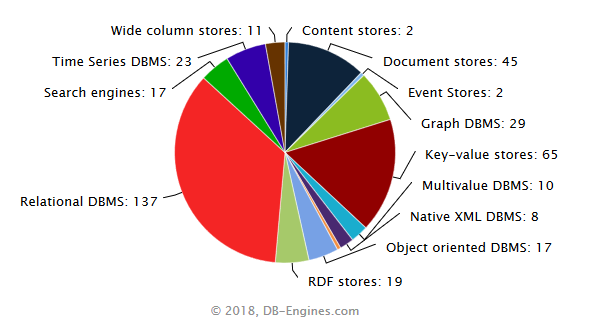
\includegraphics[width=\linewidth]{graph.png}
		\caption{Liczba DBMS wg kategorii wg \url{https://db-engines.com/en/ranking_categories}}
	\end{figure}
\end{frame}

\begin{frame}{Systematyka}
	\begin{figure}[t]
		\centering
		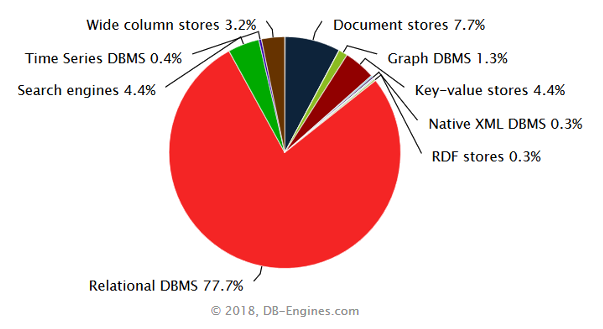
\includegraphics[width=\linewidth]{graph2.png}
		\caption{Popularność DBMS wg kategorii wg \url{https://db-engines.com/en/ranking_categories}}
	\end{figure}
\end{frame}

\section{SELECT * FROM models WHERE name = "flat";}

\begin{frame}[fragile]{Kartotekowe modele bazodanowe}
	\begin{lstlisting}
year; month; income;    gain;      currency;
2018; 01;    567432.43; 243854.04; PLN;
2018; 02;    785395.28; 387104.54; PLN;
2018; 03;    599482.41; 295859.16; PLN;
2018; 04;    257179.91; 104950.32; PLN;
	\end{lstlisting}
\end{frame}

\begin{frame}[fragile]{Kartotekowe modele bazodanowe}

	Co można zrobić?
	\begin{itemize}
		\item przesortować,
		\item przeszukać.
	\end{itemize}
	
	Czego nie można zrobić?
	\begin{itemize}
		\item zazwyczaj wymusić typu przechowywanych danych;
		\item połączyć z inna bazą danych;
		\item korzystać z indeksów, kluczy.
	\end{itemize}
\end{frame}

\begin{frame}[fragile]{Kartotekowe modele bazodanowe}

	Zalety?
	\begin{itemize}
		\item prostota obsługi,
		\item często \emph{system-agnostic},
		\item zrozumiałe nawet po bezpośrednim otwarciu.
	\end{itemize}
	
	Jak można utworzyć?
	\begin{itemize}
		\item w edytorze tekstu,
		\item w arkuszu kalkulacyjnym,
		\item w innym programie do tego przeznaczonym.
	\end{itemize}
\end{frame}

\section{SELECT * FROM models WHERE name = "hierarchical";}

\begin{frame}[fragile]{Hierarchiczne modele bazodanowe}
	\begin{lstlisting}
authors:
id; name;
1;  Richard K. Morgan
2;  Walter Jon Willians
3;  Dan Simmons

books:
id; title;               author_id
1;  Praxis;              2
2;  Rozpad;              2
3;  Wojna;               2
4;  Modyfikowany wegiel; 1
5;  Upadle anioly;       1
6;  Zbudzone furie;      1
7;  Hyperion;            3
8;  Upadek Hyperiona;    3
9;  Endymion             3
10; Triumf Endymiona;    3
	\end{lstlisting}
\end{frame}

\begin{frame}[fragile]{Hierarchiczne modele bazodanowe}
	Co można zrobić?
	\begin{itemize}
		\item połączyć rekordy z kilku tabel w drzewiastej strukturze,
		\item sortować po rekordach natywnych i zależnych,
		\item przeszukiwać po rekordach natywnych i zależnych.
	\end{itemize}
	
	Czego nie można zrobić?
	\begin{itemize}
		\item stworzyć relacji typu \emph{ma wiele},
		\item stworzyć relacji typu \emph{wiele do wielu}.
	\end{itemize}
\end{frame}

\begin{frame}[fragile]{Hierarchiczne modele bazodanowe}

	Zalety?
	\begin{itemize}
		\item prostota obsługi;
		\item czytelność schematu bazy;
		\item szybkie w porównaniu do klasycznej relacyjnej bazy danych.
	\end{itemize}

	Zastosowania?
	\begin{itemize}
		\item rejestr Windows,
		\item bankowość,
		\item telekomunikacja.
	\end{itemize}
\end{frame}

\section{SELECT * FROM models WHERE name = "relational";}

\begin{frame}{Relacyjne modele bazodanowe}
	\begin{figure}[t]
		\centering
		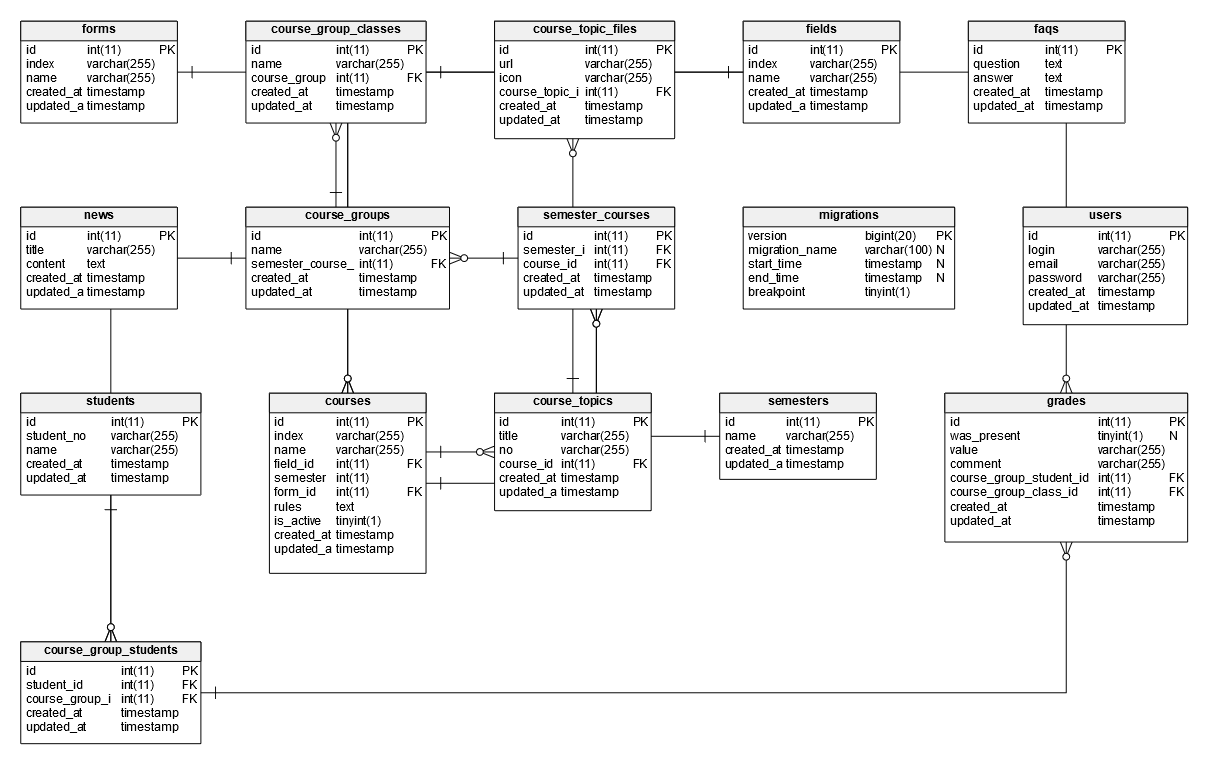
\includegraphics[width=\linewidth]{mysql.png}
	\end{figure}
\end{frame}

\begin{frame}[fragile]{Relacyjne modele bazodanowe}
	Co można zrobić?
	\begin{itemize}
		\item połączyć rekordy z kilku tabel w relacyjnej strukturze,
		\item sortować po rekordach natywnych i zależnych,
		\item przeszukiwać po rekordach natywnych i zależnych,
		\item ustanowić klucze obce, co może zabezpieczyć integralność danych,
		\item ustanowić indeksy, które pomogą przy przeszukiwaniu i sortowaniu tabel,
		\item relatywnie łatwo rozproszyć w pionie lub poziomie,
		\item korzystać z transakcji.
	\end{itemize}
\end{frame}

\begin{frame}[fragile]{Relacyjne modele bazodanowe}
	ACID, czyli
	\begin{itemize}
		\item \emph{atomicity} - niepodzielność
		\item \emph{consistency} - spójność
		\item \emph{isolation} - izolacja
		\item \emph{durability} - trwałość
	\end{itemize}
	
	Są to cechy gwarantujące poprawne przetwarzanie transakcji w (relacyjnych) bazach danych.
\end{frame}

\begin{frame}[fragile]{Relacyjne modele bazodanowe}
	Relacyjne bazy danych są obecnie najpopularniejszym modelem wykorzystywanym praktycznie wszędzie: od małych prywatnych projektów studenckich, przez produkty startupów i systemy obsługujące duże firmy, aż po korporacyjne rozwiązania.
\end{frame}

\begin{frame}{Relacyjne modele bazodanowe}
	\begin{figure}[t]
		\centering
		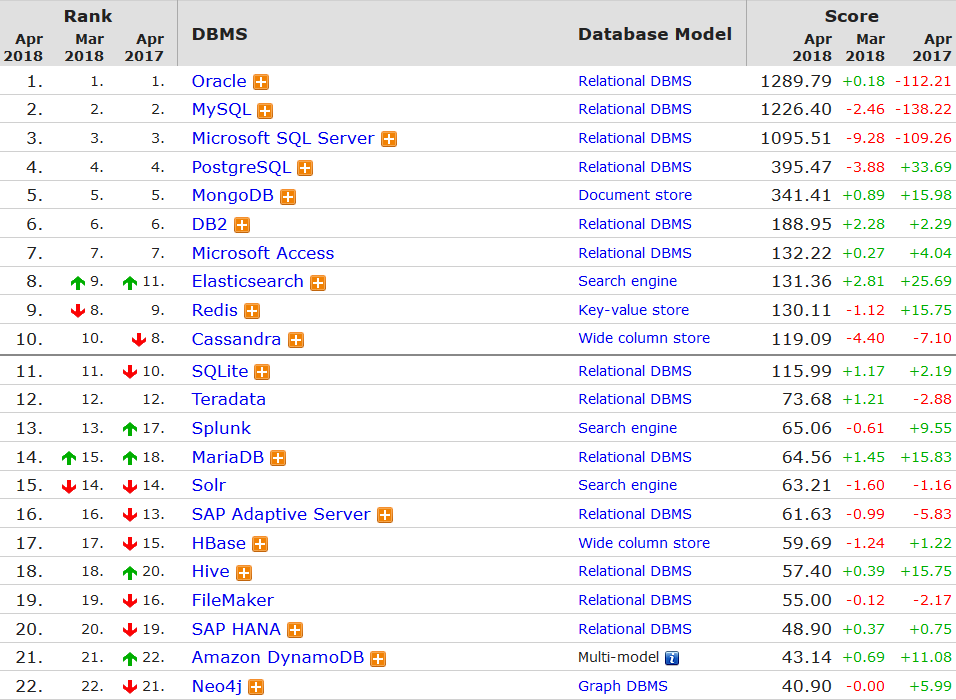
\includegraphics[width=\linewidth]{table.png}
	\end{figure}
\end{frame}

\section{SELECT * FROM models WHERE name = "object-oriented";}

\begin{frame}[fragile]{Obiektowe modele bazodanowe}
	\begin{lstlisting}
ObjectContainer oc = Db4o.openFile("database.db4o");

Author author = new Author("Cixin Liu");
Book book = new Book("Ciemny las", author);

oc.store(author);
oc.store(book);

oc.close();
	\end{lstlisting}
\end{frame}

\begin{frame}[fragile]{Obiektowe modele bazodanowe}
	Jak działają?
	\begin{itemize}
		\item są zbiorem obiektów wedle definicji obiektu wykorzystywanego języka programowania z wszystkimi tego wadami i zaletami,
		\item są przetrzymywane w formie zserializowanej lub zapisanej w inny sposób, co likwiduje potrzebę mapowania danych,
		\item są wygodne w użyciu dla progamistów znających dany język programowania,
		\item nie są szczególnie popularne przez konkurencję ze strony systemów ORM.
	\end{itemize}
\end{frame}

\begin{frame}{Obiektowe modele bazodanowe}
	\begin{figure}[t]
		\centering
		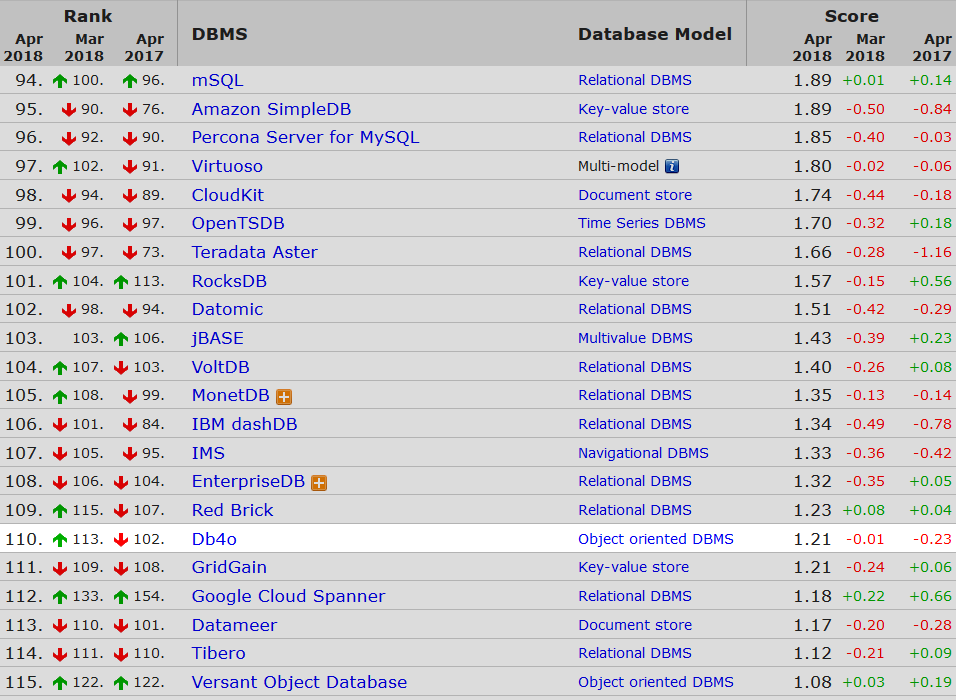
\includegraphics[width=\linewidth]{table2.png}
	\end{figure}
\end{frame}

\begin{frame}[fragile]{Obiektowe modele bazodanowe}
	Dlaczego więc w ogóle warto o nich wspominać?
	
	Przede wszystkim dlatego, że są wygodne w użyciu i zasada ich działania pokrywa się z zasadą działania systemów mapujących relacje na obiekty. Ale o tym na następnym wykładzie.
\end{frame}

\section{SELECT * FROM models WHERE name = "nosql";}

\begin{frame}[fragile]{Nierelacyjne modele bazodanowe}
	Opracowano wiele podejść do NoSQL-owych baz danych, a do najpopularniejszych należą:
	\begin{itemize}
		\item \emph{key-value}
		\item \emph{document-oriented}
		\item \emph{graph}
		\item \emph{column}
		\item \emph{multi-model}
	\end{itemize}
\end{frame}

\begin{frame}[fragile]{Nierelacyjne modele bazodanowe}
	Model klucz-wartość, często wykorzystywany jako cache, korzysta z mapy, słownika lub asocjacyjnej tablicy:

	\begin{lstlisting}
novel:54:author         // Walter Jon Williams
novel:54:originaltitle  // The Praxis
novel:54:pages          // 8
novel:54:readdatefrom   // 2018-02-07
novel:54:readdateto     // 2018-02-17
novel:54:readtitle      // Praxis
novel:54:releaseyear    // 2002
	\end{lstlisting}
\end{frame}

\begin{frame}[fragile]{Nierelacyjne modele bazodanowe}
	Co jest istotne?
	\begin{itemize}
		\item każdy klucz może pojawić się tylko raz,
		\item wykorzystywany chociażby przy procesach zakupowych lub systemach cache,
		\item łatwo znaleźć dane po kluczu, a (zazwyczaj) niekoniecznie po ich wartości,
		\item idealne do skalowania.
	\end{itemize}
\end{frame}

\begin{frame}[fragile]{Nierelacyjne modele bazodanowe}
	NoSQL-owe bazy mogą przetrzymywać ustrukturyzowane dokumenty:

	\begin{lstlisting}
{
  "author": {
    "firstname": "Walter Jon",
    "lastname": "Williams",
    "language": {
      "name": "angielski",
      "code": "en",
    }
  },
  "originaltitle": "The Praxis",
  "pages": 384,
  "readdatefrom": "2018-02-07",
  "readdateto": "2018-02-17",
  "readtitle": "Praxis",
  "releaseyear": "2002",
  "uuid": "a41b2bd7-1729-4c0d-b6a0-721ddad0a5ef",
}
	\end{lstlisting}
\end{frame}

\begin{frame}[fragile]{Nierelacyjne modele bazodanowe}
	Co jest istotne?
	\begin{itemize}
		\item pliki mogą być zapisane jako JSON, XML lub dowolny innych format,
		\item każdy dokument powinien mieć swój unikalny identyfikator,
		\item ze względu na strukturę, dane mogą być bardzo elastycznie (nie)porządkowane,
		\item łatwo skalowalne i przeznaczone do przechowywania ogromnych ilości danych.
	\end{itemize}
\end{frame}

\begin{frame}[fragile]{Nierelacyjne modele bazodanowe}
	Kolumnowe bazy składają się z plików, które przechowują po trzy zmienne: nazwę kolumny, jej wartość oraz znacznik czasowy:

	\begin{lstlisting}
{
  {
    name: "author",
    value: "Walter Jon Williams",
    timestamp: 1523819873
  },
  {
    name: "pages",
    value: 384,
    timestamp: 1523819873
  },
}
	\end{lstlisting}
\end{frame}

\section{Podsumowanie}

\begin{frame}[fragile]{HDD?}
	Najważniejsze jest zinterpretowanie potrzeb danego systemu i dobranie do nich odpowiedniego narzędzia. Żadną filozofią nie jest ślepe podążanie za trendami i próbowanie implementacji popularnych silników bazodanowych do systemów, które wcale nie potrzebują grafowego lub kolumnowego podejścia.
\end{frame}

\begin{frame}[fragile]{HDD?}
	Bazy NoSQL-owe kończą przeżywać swój złoty wiek. Zaczynają być wykorzystywane w miejscach, w których powinny być wykorzystywane, a nie praktycznie wszędzie bez żadnego uzasadnienia.
	
	W bramży istnieje żartobliwe określenie HDD - \emph{hype driven development} - które oznacza wykorzystywanie technologii, które są akurat \emph{na fali}. Przestrzegam i nie polecam takiego podejścia w warunkach komercyjnych. A w prywatnych - czemu nie?
\end{frame}

\begin{frame}{Bibliografia i ciekawe źródła}
  
	\begin{thebibliography}{9}
		
		\bibitem{ranking}
		\url{https://db-engines.com/en/ranking}
		
		\bibitem{db4o}
		\url{http://www.javaexpress.pl/article/show/DB4O__Object_Database}
		
		\bibitem{mongo}
		\url{https://www.mongodb.com/compare/mongodb-mysql}
		
		\bibitem{hdd}
		\url{https://blog.daftcode.pl/hype-driven-development-3469fc2e9b22}
		
	\end{thebibliography}

\end{frame}

\appendix

\begin{frame}[standout]
	Pytania?
\end{frame}

\begin{frame}{}

	Kod prezentacji dostępny jest w repozytorium git pod adresem \texttt{https://bitbucket.org/krewak/pwsz-ppsi} \\ \ \\

	\begin{figure}
		\centering
		\href{https://bitbucket.org/krewak/pwsz-ppsi}{
			
\includegraphics[width=.15\textwidth]{../_template/bitbucket.png}
		}
	\end{figure}
	
	Wszystkie informacje dot. kursu dostępne są pod adresem \texttt{http://pwsz.rewak.pl/kursy/4} \\ \ \\

	\begin{figure}
		\centering
		\href{http://pwsz.rewak.pl/kursy/3}{
			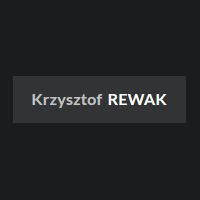
\includegraphics[width=.15\textwidth]{../_template/rewak.png}
		}
	\end{figure}

\end{frame}

\end{document}
